\documentclass{article}
\usepackage[utf8]{inputenc}  % Ensure this is loaded before biblatex
\usepackage{biblatex}  % Load the biblatex package
\addbibresource{./../Quellen/sources.bib}  % Add your .bib file


%%%%%%%%%%%%%%%%%%%%%%%%%%%%% Using Packages %%%%%%%%%%%%%%%%%%%%%%%%%%%%%%%%%%
\usepackage[a4paper, margin=2cm, top=5mm, includehead, headheight=2cm]{geometry}
\usepackage{graphicx}
\usepackage{amssymb}
\usepackage{amsmath}
\usepackage{amsthm}
\usepackage{empheq}
\usepackage{mdframed}
\usepackage{booktabs}
\usepackage{lipsum}
\usepackage{graphicx}
\usepackage{color}
\usepackage{psfrag}
\usepackage{pgfplots}
\usepackage{bm}
\usepackage{float}
\usepackage{wrapfig}
\usepackage{enumitem}
\usepackage[export]{adjustbox} % for valign option
\usepackage{caption}
\usepackage{subcaption}
\usepackage{hyperref}
\usepackage{array}
\usepackage{tocloft}
\usepackage[section]{placeins}
\usepackage[nottoc,numbib]{tocbibind}


\usepackage{emptypage}
\usepackage{fancyhdr}

\usepackage{helvet}

\renewcommand{\familydefault}{\sfdefault}

\renewcommand{\footrulewidth}{0.4pt}%
\renewcommand{\headrulewidth}{0.4pt}%

\renewcommand{\headruleskip}{3mm}
\renewcommand{\footruleskip}{4mm}

\usepackage[english,ngerman]{babel}
\usepackage[ddmmyyyy]{datetime}

\newcommand{\todayD}{\the\day.\the\month.\the\year}   

\graphicspath{{../Bilder/}}

\setlength\parindent{0pt}
\counterwithin{figure}{section}
\counterwithin{table}{section}

%%%%%%%%%%%%%%%%%%%%%%%%%%%%%%%%%%%%%%%%%%%%%%%%%%%%%%%%%%%%%%%%%%%%%%%%%%%%%%%

% Other Settings
\usepackage{xcolor}

%\pagecolor[rgb]{0,0,0} %black

%\color[rgb]{0.5,0.5,0.5} %grey

%uncomment to make the links not display the red border
%\hypersetup{
%    colorlinks,
%    citecolor=black,
%    filecolor=black,
%    linkcolor=black,
%    urlcolor=black
%}

%%%%%%%%%%%%%%%%%%%%%%%%%% Page Setting %%%%%%%%%%%%%%%%%%%%%%%%%%%%%%%%%%%%%%%
\geometry{a4paper}

\newcommand{\iu}{{i\mkern1mu}}
\newcommand*\mathinhead[2]{\texorpdfstring{$\boldsymbol{#1}$}{#2}}


\definecolor{mred}{rgb}{0.619, 0.2392, 0.3176}


%%%%%%%%%%%%%%%%%%%%%%%%%%%%%%% Title & Author %%%%%%%%%%%%%%%%%%%%%%%%%%%%%%%%
\title{AFSS - Automated Factory Storage System}
\author{Benedikt Simbürger \\
    \and Nikolaj Voglauer der allerechte \\
    \and Vincent Sonvilla \\
    \and Elena Widmann
    }

%%%%%%%%%%%%%%%%%%%%%%%%%%%%%%%%%%%%%%%%%%%%%%%%%%%%%%%%%%%%%%%%%%%%%%%%%%%%%%%

\begin{document}


\begin{figure}[h]
    \includegraphics[width=0.5\textwidth]{HTL_Moessingerstraßen_Logo.png}
    \centering
\end{figure}

\begin{center}
    \huge \textbf{HÖHERE TECHNISCHE BUNDESLEHRANSTALT} \\
    \vspace{5mm}
    \Large{KLAGENFURT, MÖSSINGERSTRASSE}

\end{center}

\vspace{7mm}

\begin{center}
    \Large{ABTEILUNG ELEKTROTECHNIK}
\end{center}

\hrule

\vspace{10mm}

\begin{center}
    \Huge \textbf{DIPLOMARBEIT} \\
    \vspace{7mm}
    \huge{Titel der Diplomarbeit Deutsch}

    \vspace{7mm}
    \huge{Automated-Factory-Storage-System}

    \vspace{7mm}
    \Large{JAHRGANG 5AHET}

\end{center}

\vspace{20mm}

\begin{flushleft}
    \bgroup
        \Large
        \def\arraystretch{1.5}
        \begin{tabular}{p{5cm}l}
            eingereicht von & Benedikt Simbürger\\
            & Vincent Sonvilla\\
            & Nikolaj Voglauer\\
            & Elena Widmann\\
            Projektbetreuer & Dipl.-Ing. Christian Sallinger
        \end{tabular}
    \egroup
\end{flushleft}
  
\vspace{7mm}
\Large
Diese Diplomarbeit entspricht den Standards gemäß dem Leitfaden zur Umsetzung der Reife- und Diplomprüfung des BMBWF in der letztgültigen Fassung.\par
\begin{flushright}
    Klagenfurt, am 04.04.2025
\end{flushright}

\newpage

\begin{figure}[h]
    \includegraphics[width=0.5\textwidth]{HTL_Moessingerstraßen_Logo.png}
    \centering
\end{figure}

\begin{center}
    \huge \textbf{EIDESSTATTLICHE ERKLÄRUNG}\\
    \vspace{7mm}
    \Large
    \begin{tabular}{p{14cm}}
        Ich versichere an Eides statt, dass ich diese Diplomarbeit
        selbstständig verfasst und keine anderen als die angegebenen
        Quellen und Hilfsmittel verwendet habe. Alle Gedanken, die im
        Wortlaut oder in grundlegenden Inhalten aus unveröffentlichten
        Texten oder aus veröffentlichter Literatur übernommen, oder mit
        künstlicher Intelligenz generiert wurden, sind ordnungsgemäß
        gekennzeichnet, zitiert und mit genauer Quellenangabe
        versehen.
    \end{tabular}

    \vspace{10mm}
    Verfasser/Verfasserin\\
    
    \vspace{40mm}
    \bgroup
        \newcolumntype{P}[1]{>{\centering\arraybackslash}p{#1}}
        \def\arraystretch{1.5}
        \begin{tabular}{P{67mm}p{14mm}P{67mm}}
            \cline{1-1}
            \cline{3-3}
            Benedikt Simbürger & & Vincent Sonvilla\\
        \end{tabular}

        \vspace{40mm}
        \begin{tabular}{P{67mm}p{14mm}P{67mm}}
            \cline{1-1}
            \cline{3-3}
            Nikolaj Voglauer & & Elena Widmann\\
        \end{tabular}
    \egroup

    \vspace*{\fill}
    \raggedleft Klagenfurt, am 04.04.2025

\end{center}

\newpage

\pagestyle{fancy}
\fancyhf{}
\fancyhf[EHL]{\includegraphics[width=0.2\textwidth]{HTL_Moessingerstraßen_Logo.png}}
\fancyhf[OHL]{\includegraphics[width=0.2\textwidth]{HTL_Moessingerstraßen_Logo.png}}

\fancyhf[EHC]{\begin{tabular}{cc}
    Simbürger & Sonvilla \\
    Voglauer & Widmann \\
\end{tabular}}

\fancyhf[OHC]{\begin{tabular}{cc}
    Simbürger & Sonvilla \\
    Voglauer & Widmann\\
\end{tabular}}

\fancyhf[EHR]{\color{mred} ELEKTROTECHNIK}
\fancyhf[OHR]{\color{mred} ELEKTROTECHNIK}

\fancyhf[EFL]{\todayD}
\fancyhf[OFL]{\todayD}

\fancyhf[EFC]{Automated-Factory-Storage-System}
\fancyhf[OFC]{Automated-Factory-Storage-System}

\fancyhf[EFR]{\thepage}
\fancyhf[OFR]{\thepage}


\newpage
\normalsize

\section*{Kurzbeschreibung}
\textcolor{blue}{
Beschreiben Sie das Projekt an dieser Stelle mit maximal zwei aussagekräftigen Sätzen, die dem Leser die Projektidee kompakt vermitteln und eine thematische Zuordnung ermögli-chen.
Die Kurzbeschreibung, im Umfang von einer A4-Seite, umfasst die wesentlichen Aspekte des Projektes in sozialer und technischer Hinsicht. Die Zielgruppe der Kurzbeschreibung sind auch Nicht-Techniker! 
Diese Beschreibung wird für Wettbewerbe und PR-Aktivitäten verwendet. Diese Inhalte sind unter dem Menüpunkt „About“ bzw. „Beschreibung“ auf der Projekthomepage dar-zustellen. Auf die Formulierung der Kurzbeschreibung sollte sehr viel Wert gelegt werden, weil viele Leser oft nur diese Seite lesen und den Rest lediglich durchblättern. Erstellen Sie die finale Kurzbeschreibung erst nach der Fertigstellung der Diplomarbeit.}

\color{blue}
\subsection*{Aufgabenstellung}
\begin{itemize}
    \item Warum ist die Themenstellung von Interesse?
    \item Was ist die vorgegebene Zielsetzung?
    \item Welche Ergebnisse sind zu erreichen?
\end{itemize}

\subsection*{Realisierung}
\begin{itemize}
    \item Von welchem Stand der Technik im Umfeld der Aufgabenstellung wurde ausgegan-gen?
    \item Welche Lösungsansätze sind grundsätzlich möglich?
    \item Warum wurde ein bestimmter Lösungsansatz gewählt?
    \item Welche experimentelle, konstruktive oder softwaretechnische Methodik wurde angewendet?
    \item Auf welche fachtheoretischen Grundlagen wurde aufgebaut?
    \item Welche wirtschaftlichen Überlegungen wurden angestellt?
\end{itemize}

\subsection*{Ergebnisse}
\begin{itemize}
    \item Worin besteht der konkrete Beitrag zur Lösung der Aufgabenstellung (Prototyp, Entwurfsplanung, Softwareprodukt, Businessplan etc.)?
    \item Kann das Ergebnis durch eine typische Grafik, ein Diagramm bzw. ein Foto illus-triert werden?
    \item Kann in die Vollversion der Diplomarbeit Einsicht genommen werden?
\end{itemize}

\color{black}
\vspace*{\fill}
\section*{}

\bgroup
    \def\arraystretch{1.5}
    \begin{tabular}{p{48mm}p{113mm}}
        \textbf{Kurztitel:} & \textcolor{blue}{Kurztitel der Diplomarbeit (etwa. 30 Zeichen)}\\
        \textbf{Schlüsselwörter:} & \textcolor{blue}{Maximal fünf aussagekräftige und durch Kommas getrennte Schlüsselwörter, welche die Inhalte möglichst gut beschreiben.}
    \end{tabular}
\egroup

\newpage

\section*{Abstract}
\textcolor{blue}{Die Kurzbeschreibung in englischer Sprache sollte sinngemäß exakt der Kurzbeschreibung in deutscher Sprache entsprechen, siehe Abschnitt „Kurzbeschreibung“.}

\vspace*{\fill}
\section*{}

\bgroup
    \def\arraystretch{1.5}
    \begin{tabular}{p{48mm}p{113mm}}
        \textbf{Short title:} & \\
        \textbf{Keywords:} & 
    \end{tabular}
\egroup

\newpage
\tableofcontents
\newpage
\section{Einleitung}

\color{blue}
Mit der Einleitung beginnt der inhaltliche Teil der Arbeit. Es ist die Wahl der Themenstel-lung und das Interesse an dieser Themenstellung zu begründen.\\
Beschreiben Sie die Ausgangslage und die vom Auftraggeber stammende Problemstel-lung. Leiten Sie daraus die konkrete Aufgabenstellung und Zielsetzung des Gesamtpro-jekts ab. Geben Sie einen kurzen Überblick über das fachliche und wirtschaftliche Projekt-umfeld. Stellen Sie gegebenenfalls Ihre Kooperationspartner (Firma, Kontaktpersonen, Kontaktdaten, Zuständigkeit, etc.) dar. \\
Die Leserinnen und der Leser bekommen durch dieses Kapitel einen Gesamteindruck über die vorliegende Diplomarbeit. An dieser Stelle kann es hilfreich sein, das Zusammenwirken unterschiedlicher Komponenten des Gesamtsystems grafisch darzustellen, z.B. mittels eines Blockschaltbildes der Systemstruktur oder ähnlicher Darstellungsformen. In der Sys-temübersicht sollten bereits die Zuständigkeitsbereiche der einzelnen Projektmitglieder ausgewiesen sein und im Text auch oberflächlich beschrieben werden, siehe Abbildung~\ref{Systemstruktur}.\\

\begin{figure}[h]
    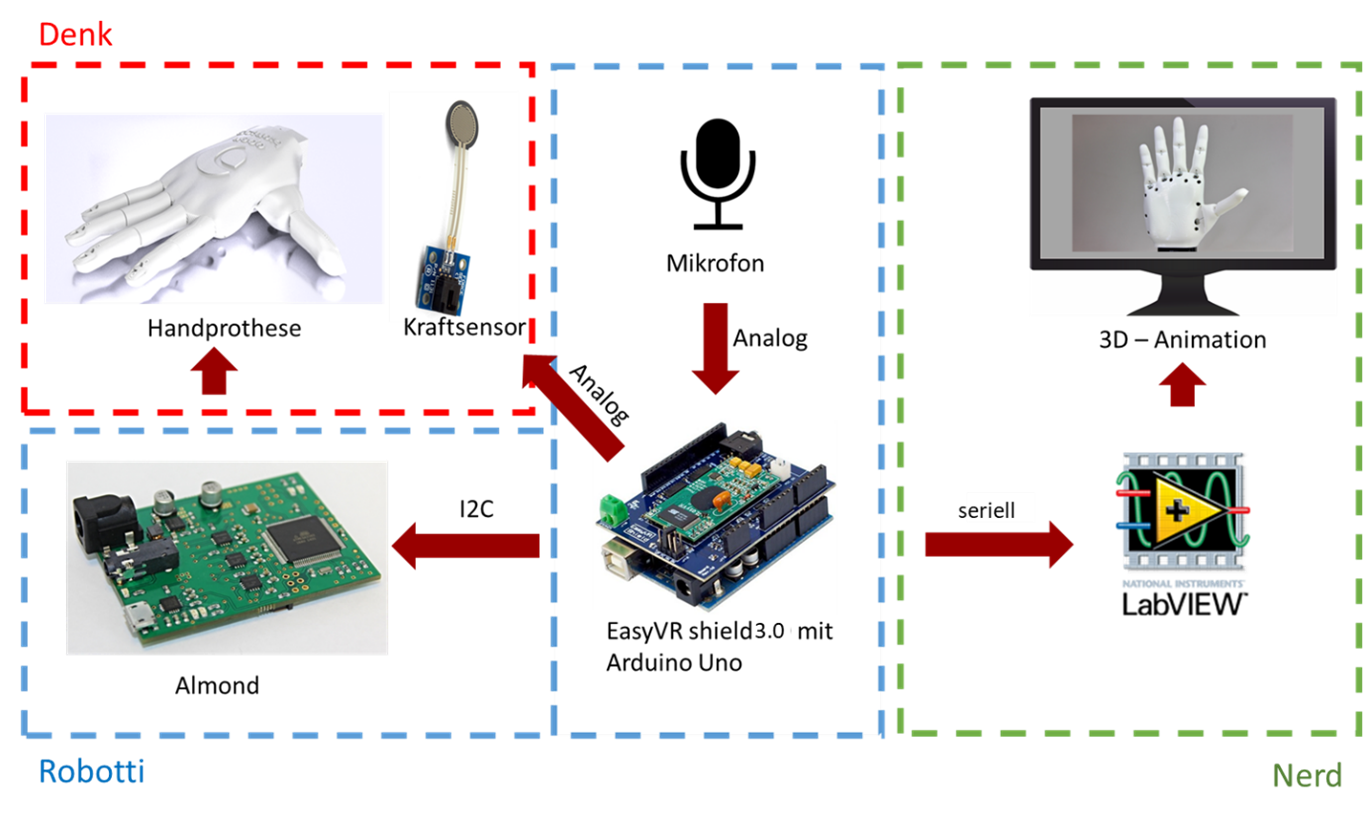
\includegraphics[width=1\textwidth]{Systemstruktur.png}
    \centering
    \caption{Systemstruktur}
    \label{Systemstruktur}
\end{figure}

Stellen Sie kurz die in der Arbeit behandelten Themen vor und verweisen Sie auf die ent-sprechenden Abschnitte in der Diplomarbeit.\\
\color{black}

\subsection{Vision}
\subsection{Projektziel}
\subsection{Kooperationspartner}

\newpage
\section{Grundlagen und Methoden}
\color{blue}
Dieses Kapitel ist der gemeinsame Hauptteil Ihrer Diplomarbeit und ist üblicherweise in mehrere Unterkapitel unterteilt.\\
Beschreiben Sie die Ist-Situation des Standes der Technik und darauf aufbauend erläutern Sie mögliche Lösungsansätze, die zur Umsetzung in Frage kommen. Begründen Sie die ge-wählten Methode und Lösungsansätze.\\
In diesem Kapitel werden auch die Grundlagen behandelt, die für das gesamte Projekt essentiell sind und nicht einem einzigen Funktionsblock alleine zugeordnet werden kann.\\
Es ist die Gesamtsicht, die zur Lösung Ihrer Aufgabenstellung führt, darzulegen. Notwen-dige Schnittstellen zwischen den einzelnen Modulen können anhand eines detaillierteren Gesamtblockschaltbildes beschrieben werden (hier nicht dargestellt). \\
An dieser Stelle ist die Produkt- und die daraus abgeleitete Projektstruktur in From eine Scrum-Projektplans darzulegen, zu beschreiben und zu argumentieren.\\
Der Produktstrukturplan (PdSP) enthält die wichtigsten Systemkomponenten (Hard-ware/Software) des Gesamtsystems, weshalb in den Blöcken Hauptwörter stehen, die die Komponenten bezeichnen, siehe Abbildung~\ref{Produktstruktur}. \\
Der Scrum-Projektplan beschreibt den geplanten Projektablauf, siehe Fehler! Verweisquel-le konnte nicht gefunden werden..  Die Vorlage für den Scrum-Plan und eine Beschreibung zum Aufbau befindet sich in der DA-PowerPoint-Vorlage. An dieser Stelle ist der Scrum-Plan nur bis zur Story-Ebene darzustellen, sodass die (grobe) Projektplanung beschrieben werden kann. Aus der Beschreibung soll die wichtigsten Arbeitspakete und die Verant-wortlichkeiten der Teammitglieder eindeutig hervorgehen. Die Epics (etwa 4 Wochen) und Stories (etwa 2 Wochen) sind kurz zu beschreiben. Die konkreten Tätigkeiten werden als Tasks bezeichnet und befinden sich in der dritten Ebene. Task-Beschreibungen müssen stets ein Verb beinhalten, z.B. „Platine bestücken und testen“. Der vollständigen Scrum-Projektplan inklusive der Tätigkeiten wird allerdings erst in Kapitel 8.1.2 eingefügt.\\
Um die Lesbarkeit der Darstellungen zu gewährleisten, kann es sinnvoll sein, diese im Querformat in Dokument einzufügen oder mehrere Teilbereiche in separaten Abbildun-gen darzustellen.\\

\begin{figure}[h]
    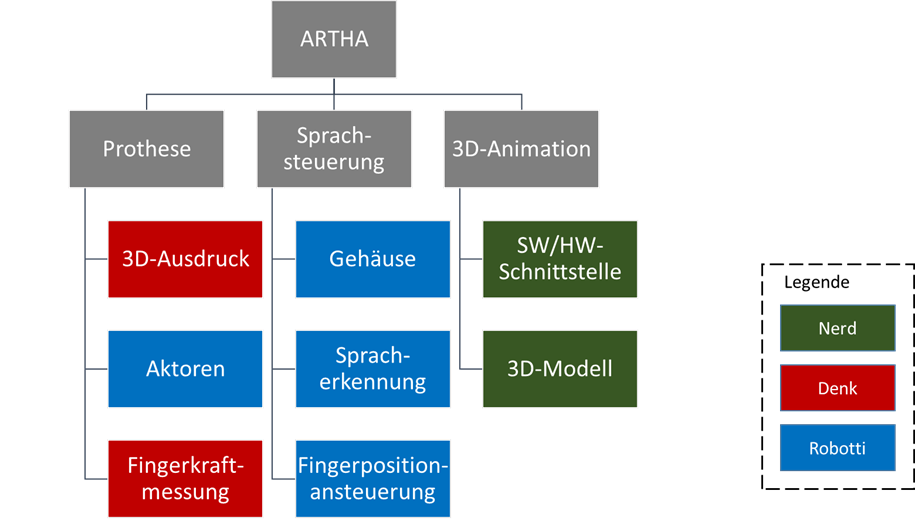
\includegraphics[width=1\textwidth]{Produktstruktur.png}
    \centering
    \caption{Produktstruktur}
    \label{Produktstruktur}
\end{figure}

Die Überschriften der nachfolgenden Unterkapitel stellen lediglich Platzhalter dar und können durch spezifische, aussagekräftigere Titel ersetzt werden (Formatierung als Über-schrift!).\\
2.1 Ist-Situation / Stand der Technik\\
2.2 Lösungsmethoden / Lösungsansatz\\
2.3 Grundlagen für das Gesamtprojekt\\
2.4 Schnittstellen zwischen den Modulen\\
2.5 Produktstrukturplan (PdSP)\\
2.6 Scrum-Projektplan (Epics und Stories)

\begin{figure}[h]
    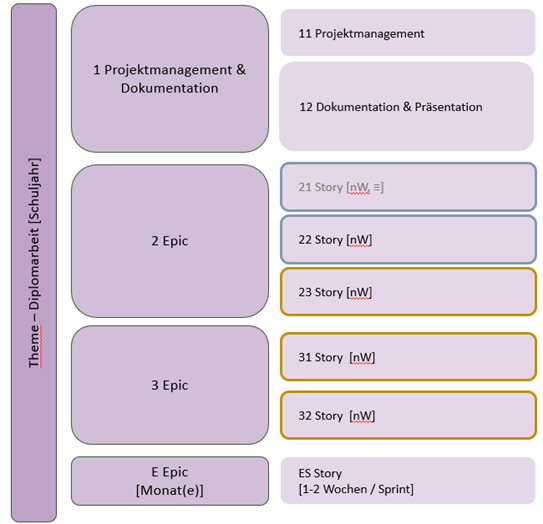
\includegraphics[width=0.8\textwidth]{Scrum_Projektplan.png}
    \centering
    \caption{Scrum Projektplan}
\end{figure}

\color{black}
\newpage
\section{Titel der Individuellen Themenstellung (Benedikt Simbürger)}
\color{blue}
Jedes Teammitglied bearbeitet die individuell vereinbarte Zielsetzung, im Kontext der Gesamtaufgabenstellung, eigenständig. Der individuelle Teil sollte pro Teammitglied ei-nen Seitenumfang von etwa 25 bis 30 Seiten umfassen.\\
Der Titel der individuellen Aufgabenstellung entspricht der Bezeichnung Ihrer „Individuel-len Themenstellung“, siehe Diplomarbeitsdatenbank (Genehmigung). Achtung, in der Kopfzeile der individuellen Kapitel wird ausschließlich der Name des jeweiligen Teammit-glieds (Urheber) angegeben!\\
Beschreiben Sie an dieser Stelle ausführlich die konkrete Aufgabenstellung zu Ihrer indivi-duellen Zielsetzung. Die Überschriften der nachfolgenden Unterkapitel stellen lediglich Platzhalter dar und können durch spezifische, aussagekräftigere Titel ersetzt werden. Die Arbeit sollte allerdings stets die drei Aspekte (Grundlagen/Methoden, Realisie-rung/Implementierung, Ergebnisse) in einer angemessenen Art und Weise beinhalten.\\

\begin{itemize}
    \item Eine reine Abschreibübung theoretischer Inhalte (copy and paste) wird nicht ange-strebt.
    \item Eine möglichst solide technische Darstellung der eigenen Arbeit hingegen ist äu-ßerst erwünscht.
    \item Grobstruktur der individuellen Lösung (inkl. Begründung): Blockschaltbild \(\rightarrow\) Schaltung  Flussdiagramme/Klassendiagramme \(\rightarrow\) Quellcode (auszugsweise) \textbar Anforde-rung \(\rightarrow\) Datenbankschema \textbar etc.
    \item Detaillierte Beschreibung der konkreten Umsetzung mit Referenzen auf relevanten Quellen (Primärliteratur/ Webseiten): Schaltungsentwicklung und Simulationen, Al-gorithmen, Messreihen und Auswertungen.
\end{itemize}

\section*{Gliederung der Arbeit und Inhalte}
Der individuelle Teil kann und soll nach eigenem Ermessen gestaltet werden. Ein Leitfaden für einen guten Stil und eine gute Dokumentstruktur finden Sie in Kapitel 7. Die Über-schriften sollten nicht zu allgemeingültig, sondern möglichst spezifisch und aussagekräftig für ihre Arbeit, gewählt werden. Inhaltlich sollten die folgenden Punkte in ihrer Arbeit enthalten sein:

\begin{itemize}
    \item Beschreiben Sie kurz, zum Beispiel den Stand der Technik, die Lösungsalternativen und begründen Sie die Wahl des Lösungsansatzes, die auf Ihre individuelle Zielset-zung zutrifft. 
    \item Beschreiben Sie alle theoretischen Betrachtungen und praktischen Tätigkeiten, die Sie während der Umsetzung Ihrer individuellen Zielsetzung durchgeführt haben. An dieser Stelle präsentieren Sie den eigentlichen Hauptteil Ihrer „Arbeit“.
\end{itemize}

\textbf{Theoretischer Teil:} Analysen von Markt/Systemen/Baugruppen/Sensoren/Bauteilen, Lösungswege, Berechnungen, Simulationen, Schaltungen, Funktionsbeschreibungen, Schnittstellen, Codeauszü-ge. \\
\textbf{Praktischer Teil:} Messaufgaben, Aufbauten, Messschaltungen, Fotos, Tabellen, Di-agramme, Tests, Ergebnisse, Vergleiche, Interpretationen\\
Besteht Ihre Arbeit aus mehreren Komponenten, ist es im Regelfall sinnvoll diese in je-weils eigenen Unterkapiteln zu behandeln. Die obigen Punkte würden sich in diesem Fall komponenten-spezifisch in den einzelnen Unterkapiteln „wiederholen“. \\
Jede Arbeit sollte mit einem Kapitel “Konklusion“ (maximal eine Seite) enden, in welcher die tatsächlich erzielten Ergebnisse kompakt zusammengefasst werden (Ergebnisse, Ver-gleiche, Interpretationen) und ein Ausblick für eine mögliche zukünftige Weiterentwick-lung des Projekts gegeben wird (Ausständiges, offene Probleme, Erweiterungen, etc.).\\
Die Überschriften der nachfolgenden Unterkapitel stellen lediglich Platzhalter dar und können durch spezifische, aussagekräftigere Titel ersetzt werden (Formatierung als Über-schrift!).\\
3.1 Aufgabenstellung\\
3.2 Grundlagen / Methoden\\
3.3 Realisierung / Implementierung\\
3.4 Ergebnisse / Konklusion\\

\color{black}
\newpage
\section{Titel der Individuellen Themenstellung (Vincent Sonvilla)}

\newpage
\section{Titel der Individuellen Themenstellung (Nikolaj Voglauer)}

\newpage
\section{Titel der Individuellen Themenstellung (Elena Widmann)}

\newpage
\section{Anhang}
\textcolor{blue}{Im Anhang befinden sich weitere Detailinformationen des Projekts wie\\
•	Datenblattauszüge, Fertigungsunterlagen (PCB-Layouts, Gehäusezeichnungen, 3D-Druckunterlagen, Montageanleitungen,…) etc.\\
•	sämtliche geforderten Projektmanagementdokumente\\
•	ein Businessplan (optional)
}

\subsection{Projektmanagement}
\textcolor{blue}{In diesem Kapitel soll auf das Projektmanagement des Projektes eingegangen werden. Zu Beginn empfiehlt es sich, die einzelnen Bereiche des Projektmanagements zu erklären und anschließend in einzelnen Kapiteln zu behandeln.}

\subsubsection{Aufgabenstellung des Gesamtprojekts}
\textcolor{blue}{Fügen Sie an dieser Stelle den Text der genehmigten Aufgabenstellung ein, der in die Diplomarbeitsdatenbank  eingegeben wurde.}

\subsubsection{Scrum-Projektplan}
\textcolor{blue}{Fügen Sie hier den vollständigen Scrum-Projektplan, wobei die Nummern der Tasks mit der Arbeitszeitaufzeichnung übereinstimmen müssen. Der Scrum-Projektplan kann auf mehrere Seiten aufgeteilt werden.}

\bgroup
    \centering
    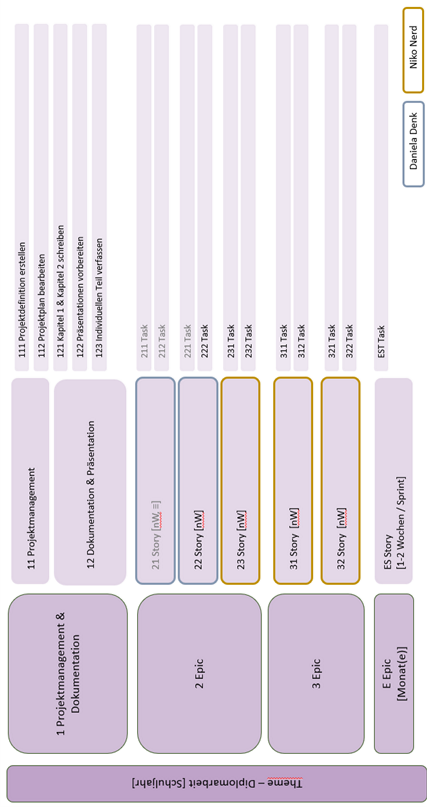
\includegraphics[width=0.6\textwidth]{Scrum_Projektplan_mit_Tasks.png}
    \captionof{figure}{Scrum Projektplan mit Tasks}
\egroup

\newpage
\subsubsection{Terminplanung}

\newpage
\subsection{Inbetriebnahme}
\color{blue}
Nachdem typische Projekte aus mehreren Komponenten bestehen, ist es oft nicht trivial die einzelnen Komponenten korrekt zu konfigurieren und das Gesamtsystem in Betrieb zu nehmen. In diesem Kapitel soll eine vollständige, präzise und trotzdem möglichst kompak-te Anleitung zur Inbetriebnahme des Systems dargelegt werden. Die Schritte sollen in dem Detailgrad beschrieben werden, dass ein durchschnittlicher Schüler des vierten Jahrganges das Projekt in Betrieb nehmen kann. Exemplarisch sollten Punkte wie die folgenden be-handelt werden – die Aufzählung ist nicht vollständig):
\begin{itemize}
    \item Treiberinstallationen und Systemkonfigurationen
    \item Zu empfehlen wäre bei Server-Installationen ein Setup-Script, welches auf einem vordefinierten Docker-container aufbaut.
    \item Welche Schritte sind notwendig, um das Projekt mit dem vorhandenen Code / Schaltplänen (auf GIT, CD, Netzlaufwerk, etc.) in Betrieb zu nehmen.
    \item Bei Schaltungen mit mehreren Platinen muss beschrieben werden, wie diese mit-einander verbunden werden müssen.
\end{itemize}
\color{black}

\newpage
\subsection{Kostenaufstellung}
\textcolor{blue}{Für die Kalkulation im Gesamtprojekt sind folgende Kosten zu erfassen: \\
•	Kosten für Material (Hard- und Software)\\
•	externe Kosten (z.B.: Zukauf von Sensoren, Funkmodule, spezielle Entwicklungsum-gebungen, etc.) 
}
\begin{figure}[h]
    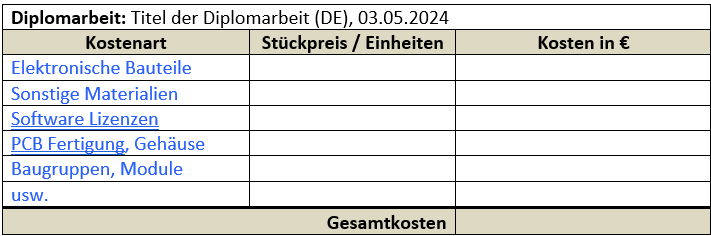
\includegraphics[width=0.8\textwidth]{Kostenaufstellung.png}
    \centering
    \caption{Kostenaufstellung}
\end{figure}

\newpage
\subsection{Besprechungsprotokolle}
\textcolor{blue}{Eine entsprechende Vorlage wird auf den Schulrechner in Form einer Word-Vorlage be-reitgestellt. Scannen Sie die vier Besprechungsprotokolle (laut Vorlage) ein und fügen Sie diese nachfolgend an (eine A4-Seite pro Protokoll)\\
Protokolle zu den einzelnen Iterationen:\\
•	Vorprojektphase\\
•	Iteration 1\\
•	Iteration 3\\
•	Iteration 5\\
Die Termine und Inhalte/Projektstatus entsprechen denen der Iterationspräsentationen.
}

\newpage
\subsection{Arbeitsnachweis}
\textcolor{blue}{Jedes Teammitglied (Schüler/in) hat einen vollständigen Arbeitszeitnachweis, der außer-halb des Unterrichts verrichteten Tätigkeiten, in tabellarischer Form zu erbringen. \\Eine entsprechende Vorlage wird auf den Schulrechner in Form einer Excel-Vorlage bereitgestellt.}

\newpage
\subsection{Wettbewerbe}
\textcolor{blue}{Teilnahme und Erfolge bei Wettbewerben.}

\newpage
\subsection{Businessplan (optional)}
\textcolor{blue}{Halten Sie sich, was die Struktur des Businessplanes angeht, an die Angaben, die Sie im WIRE-Unterricht bekommen. Das Anfügen eines Businessplans ist durch den/die WIRE Lehrer/in vorab zu genehmigen.}

\newpage
\addcontentsline{toc}{section}{Literaturverzeichnis}
\printbibliography[title=Literaturverzeichnis]

\newpage
\renewcommand{\cftfigpresnum}{Abb. }
\setlength{\cftfignumwidth}{2cm}
\listoffigures

\newpage

\renewcommand{\cfttabpresnum}{Tab. }
\setlength{\cfttabnumwidth}{2cm}
\listoftables

\end{document}